\documentclass[12pt]{article}

\usepackage[a4paper, left = 2cm, right = 2cm, top = 2cm, bottom = 2cm]{geometry}

\usepackage{amsmath}
\usepackage{amssymb}

\usepackage{graphicx}

\usepackage{listings}
\usepackage{xcolor}
\lstset{
	language = Python,
	backgroundcolor=\color{black!5}, % set backgroundcolor
}

\renewcommand{\baselinestretch}{1.5}

\renewcommand\thesection{\arabic{section}.}

\usepackage{tocloft}
\cftsetindents{section}{0em}{2em}
\cftsetindents{subsection}{0em}{2em}
\renewcommand\cfttoctitlefont{\hfill\Large\bfseries}
\renewcommand\cftaftertoctitle{\hfill\mbox{}}
\setcounter{tocdepth}{2}

%\title{CS553: Cryptography \\
%		Assignment 2 - Solutions\\\vspace{1cm}}
%\author{Rohit Das (11910230)}

\begin{document}
%\maketitle
%\newpage
\begin{titlepage}
\centering
\vspace*{\fill}
\huge CS553: Cryptography\\
\LARGE Assignment 2: Solutions\\
\Large Rohit Das (11910230)\\\vspace{0.8cm}
\today
\vspace*{\fill}
\end{titlepage}

\section{How Many Keys?}
\begin{large}
$r = 23$ (formed from $2nd$ and $3rd$ digits of roll number)\\
$\therefore \mathbb{Z}^{+}_{23} = \{0,1,...,22\}$\\
Let $K$ be the set of possible keys, such that $\forall	k \in K$, gcd($r,k$) $= 1$.\\
So, given $r = 23$, $K = \{1,2,...,22\}$.\\
$\mathbf{\therefore |K| = 22}$.
\end{large}

\section{Euler Phi Function}
\begin{large}
Euler Phi Function, also known as Euler's totient function, returns the count of integers less than and relatively prime to n. It is denoted by $\phi(n)$.\\
For prime positive integers, $\phi(n) = (n - 1)$. For other positive integers, if $n = pq$, where p,q $\in \mathbb{Z}^{+}$ and prime, $\phi(n) = (p - 1)(q - 1)$.\\
The number of keys, $|K|$, for an Affine Cipher defined over $\mathbb{Z}^{+}_{r}$ can be easily obtained by simply using Euler's totient function $\phi(r)$.\\
Since our $r$ is prime, $\phi(r) = (r - 1) = 22$.
\end{large}

\section{Bijection}
\begin{large}
Given $X = \{x_{1}, x_{2},..., x_{n}\}, Y = \{y_{1}, y_{2},..., y_{n}\}$ and $|X| = |Y|$.\\
Also given, $f: X \to Y$ is injective, i.e. $\forall$ $x \in X$, $f(x)$ is unique, or $f(x)$ is a one-to-one function. So naturally, $|X| \le |Y|$.\\
But, we know $|X| = |Y|$, meaning, $\forall$ $y \in Y$, $\exists$ $x \in X$, s.t. $f(x) = y$. Hence, $f$ is also surjective, i.e. onto.\\
\begin{figure}[h!]
\centering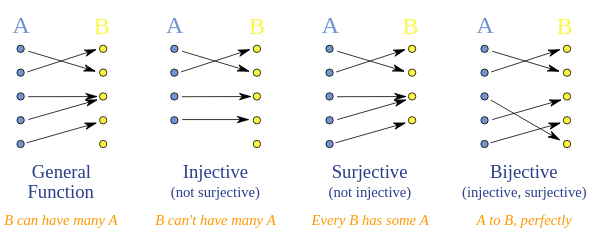
\includegraphics[width = 0.75\linewidth]{./images/HW2_1.png}
\end{figure}
$\therefore f$ is a bijection (Proved).
\end{large}

\section{Euclidean GCD}
Python code (Python3): Euclidean\textunderscore gcd.py
\lstinputlisting[language = Python, showstringspaces=false]{./python_code/Euclidean_gcd.py}

\section{Involutory Key}
\begin{large}
\subsection{Proof of involutory key}
Given an Affine Cipher over $\mathbb{Z}_{m}$ with $K = (a,b)$.\\
Let $e_{K}(x) = (ax + b)$ mod m, $d_{K}(x) = a^{-1}(x - b)$ mod m be the encryption and decryption function respectively.\\
\underline{Proof 1}: Assuming key K is involutory, i.e. $d_{K}(x) = e_{K}(x).......(1)$, to prove\\ $a^{-1}$ mod m $ = a$, and $b(a + 1) \equiv$ $0$ mod m.\\
From $(1)$, $(ax + b)$ mod m $=$ $a^{-1}(x - b)$ mod m,\\
$\implies$ $(ax + b)$ mod m = $(a^{-1}x - a^{-1}b)$ mod m\\
$\therefore$ $a$ $\equiv$ $a^{-1}$ mod m$....(2)$, and\\ $b$ $\equiv$ $-a^{-1}b$ mod m$....(3)$ $[\because$ two functions $ax + b$ and $cx + d$ are equal if their coefficients are equal, i.e. a = c and b = d].\\
From $(2)$, we get $a \equiv a^{-1}$ mod m (Proved).\\
From $(3)$, we get $ab \equiv -b$ mod m,\\
$\implies$ $b(a + 1) \equiv 0$ mod m (Proved)\\
\underline{Proof 2}: Assuming $a \equiv a^{-1}$ mod m$...(4)$, and $b(a+1) \equiv 0$ mod m, to prove K is involutory, i.e. $e_{K}(x) = d_{K}(x)$\\
$b(a + 1) \equiv 0$ mod m\\
$\implies ba \equiv -b$ mod m, $\implies b \equiv -a^{-1}b$ mod m$...(5)$\\
Putting $(4)$ and $(5)$ in $e_{K}(x)$, we get\\
$e_{K}(x) = (ax + b)$ mod m = $\{a^{-1}x$ mod m  + ($-a^{-1}b)$ mod m\} mod m\\
= $a^{-1}(x - b)$ mod m = $d_{K}(x)$ $\implies$ Key K is involutory\\
$\therefore$ The above two proofs prove that Key K is involutory iff $a \equiv a^{-1}$ mod m, and $b(a + 1) \equiv 0$ mod m.(Proved)
\subsection{Number of involutory keys}
For an Affine Cipher defined over $\mathbb{Z}_{15}$, possible values for a, such that $a = a^{-1}$ mod m are \{$1,4,11,14$\}(using $a^{2}$ mod $15$). For each value of a, possible values of b such that $b(a + 1) \equiv 0$ mod n follow:\\
For $a =  1$, $b$ (1 + 1) = $2b$, meaning, only possible value for b $\in$ $\mathbb{Z}_{15}$ is 0. $|b| = 1$\\
For $a = 4$, $b$ (4 + 1) = $5b$. So, $b = \{0,3,6,9,12\}$. $|b| = 5$.\\
For $a = 11$, $b$ (11 + 1) = $12b$. $b = \{0,5,10\}$. $|b| = 3$.\\
For $a = 14$, $b$ (14 + 1) = $15b$. $b$ can take any value from $\mathbb{Z}_{15}$. $|b| = 15$.\\
$\therefore$ Total no. of involutory keys = 1 + 5 + 3 + 15 = \textbf{24}.
\end{large}
\end{document}